% Interspeech-style two-column manuscript.
%
% The official `interspeech.sty` is not redistributable and is not bundled here;
% the geometry, type size and section styling below reproduce the Interspeech
% layout (A4, two 80 mm columns, 10 mm gutter, 9 pt Times) so the paper
% compiles anywhere with Tectonic. For an actual submission, drop the official
% class file in and delete the geometry/style block marked below.

\documentclass[a4paper,9pt,twocolumn]{extarticle}

\usepackage[T1]{fontenc}
\usepackage[utf8]{inputenc}
\usepackage{newtxtext,newtxmath}
\usepackage{graphicx}
\usepackage{booktabs}
\usepackage{amsmath}  % amssymb is provided by newtxmath; loading it clashes on \Bbbk
\usepackage{multirow}
\usepackage{array}
\usepackage{caption}
\usepackage[colorlinks=true,linkcolor=black,citecolor=black,urlcolor=blue]{hyperref}
\usepackage{url}
\usepackage{microtype}
\usepackage{balance}

% ------------------------------------------------- Interspeech-like geometry
\usepackage[a4paper,left=20mm,right=20mm,top=25mm,bottom=37mm,
            columnsep=10mm]{geometry}
\setlength{\parindent}{1em}
\setlength{\parskip}{0pt}
\captionsetup{font=small,labelfont=bf,skip=4pt}
\captionsetup[table]{skip=3pt}
\usepackage{titlesec}
\titleformat{\section}{\normalsize\bfseries}{\thesection.}{0.5em}{}
\titleformat{\subsection}{\small\bfseries}{\thesubsection.}{0.5em}{}
\titleformat{\subsubsection}{\small\itshape}{\thesubsubsection.}{0.5em}{}
\titlespacing*{\section}{0pt}{7pt plus 2pt minus 1pt}{3pt}
\titlespacing*{\subsection}{0pt}{5pt plus 1pt minus 1pt}{2pt}
\titlespacing*{\subsubsection}{0pt}{4pt plus 1pt minus 1pt}{2pt}
% -------------------------------------------------- end geometry/style block

\newcommand{\ft}[1]{\texttt{\footnotesize #1}}
\newcommand{\scsix}{\ft{spectral\_contrast\_6\_mean}}

\title{\vspace{-6mm}\Large\bfseries Thresholds Survive, Products Collapse:\\
Model Family Governs Robustness to Perceptual Coding\\
in Speech Emotion Recognition}

\author{\normalsize Akshath R \\[1mm]
\small Independent Researcher \\
\small \ft{akshath.r333@gmail.com}}
\date{}

\begin{document}
\twocolumn[
\begin{@twocolumnfalse}
\maketitle
\vspace{-6mm}
\begin{abstract}
\noindent
Speech emotion recognition (SER) is validated on uncompressed audio and
deployed on coded audio. We measure what that substitution costs and find the
answer is not a property of the codec. Fifteen classifiers --- fourteen
scikit-learn models and a neural network --- are trained on 436 named acoustic
descriptors from CREMA-D under a speaker-independent split, then served MP3 and
MP4/AAC at 64\,kbps. Under MP3 the outcome is categorical rather than graded:
every model that thresholds a feature value stays within 1.4 points of its
clean balanced accuracy, while every model that multiplies one loses 11.7 to
38.3 points. The two families do not overlap. Because the features are named
the mechanism is legible: perceptual bit allocation abandons the top octave,
and one descriptor of that octave arrives 38.6 training standard deviations out
of range. Masking that single column recovers 97.9\,\% of an RBF-SVM's loss and
92.3\,\% of the network's at no cost on clean audio, so the failure is
covariate shift on an identifiable channel rather than lost emotional
information. Attribution stability follows the same family split, and we retain
two negative results constraining how such stability should be used.
\end{abstract}
\vspace{2mm}
\noindent\textbf{Index Terms}: speech emotion recognition, perceptual audio
coding, covariate shift, explainable AI, model robustness
\vspace{4mm}
\end{@twocolumnfalse}
]

\section{Introduction}
Audio rarely reaches an inference endpoint in the representation in which it was
captured. Contact-centre archives hold MP3, streaming clients negotiate AAC or
Opus, and a clip may be transcoded several times between microphone and model.
Evaluation practice runs the other way: SER corpora are distributed as
uncompressed WAV and read directly from disk.

The gap is usually dismissed on a reasonable-sounding argument. Any ingestion
path decodes to linear PCM before feature extraction, so the delivery format is
an implementation detail. Where the assumption has been tested, it has been
tested as an average: Reddy and Vijayarajan~\cite{reddy2020compression} report
codec effects on SER that are real but modest and front-end-dependent.

We show that the average is the wrong summary, because the underlying
distribution is bimodal. Training fifteen models on one feature table, one
split, and one set of labels, and serving them MP3 at 64\,kbps, produces a
clean partition: seven models lose essentially nothing and eight lose between
a fifth and two thirds of their headroom above chance. Nothing about the codec
distinguishes the two groups --- they receive bit-identical inputs. What
distinguishes them is how the decision rule consumes a feature value. A tree
asks whether a descriptor exceeds a threshold, and the answer is unchanged
whether it reads 16.4 or 46.4; a linear, kernel, or neural model multiplies
that excursion straight into its decision function.

Because the 436 features carry acoustic names, the argument does not stop at
the observation. We locate the contaminated channel, verify it is the one the
encoder abandons, repair the failure by masking it, and confirm on clean audio
that the masked column was never load-bearing evidence.

\medskip\noindent\textbf{Contributions.} We report a model-family split in
codec robustness under MP3 with no overlap between the two families and a
mechanism stated in acoustic terms (\S\ref{sec:family}); a diagnosis-and-repair
procedure that recovers almost the entire collapse from a single column, with a
clean-audio control ruling out the trivial explanation (\S\ref{sec:repair});
cross-format attribution stability for six model families on identical inputs,
including two negative results retained rather than smoothed
(\S\ref{sec:xai}); and a container control confirming that the operational risk
localises entirely to the codec.

\section{Related Work}
\textbf{Coding and speech tasks.} Degradation of speech systems under lossy
coding is documented but shallowly characterised. The most consequential result
comes from neural codec benchmarking: Wu et al.~\cite{wu2024codecsuperb} show
that signal-domain fidelity metrics fail to predict retention of task-relevant
information, so a codec can score well under reconstruction error while
discarding paralinguistic content. We therefore report the induced feature
shift and the model behaviour as separate quantities.

\textbf{Interpretability.} Post-hoc attribution rests on a small set of
workhorses: local surrogates~\cite{ribeiro2016lime}, Shapley-value
attribution~\cite{lundberg2017shap} with an exact algorithm for tree
ensembles~\cite{lundberg2020treeshap}, and for differentiable models
path-integral~\cite{sundararajan2017ig} and reference-based~\cite{shrikumar2017deeplift}
decompositions, available in consolidated form~\cite{kokhlikyan2020captum};
surveys map the space~\cite{guidotti2018survey}. Rudin~\cite{rudin2019stop}
argues that for high-stakes decisions the post-hoc layer should be replaced by
an intrinsically interpretable model, a position our \S\ref{sec:leaderboard}
result speaks to directly and unfavourably. Transfer of these methods to audio
is contested: Haunschmid et al.~\cite{haunschmid2020audiolime} argue that
transplanting image-segmentation logic onto time--frequency representations
yields components with no perceptual correlate, and related critiques extend to
music and to speech emotion
specifically~\cite{becker2018audiomnist,sotirou2024musiclime,nasr2025beyond}.
We sidestep the objection by attributing over named acoustic descriptors in the
tradition of GeMAPS~\cite{eyben2016gemaps} and
openSMILE~\cite{eyben2010opensmile}, where every unit of attribution has a
phonetic reading by construction.

\textbf{Attribution fragility.} Attributions can be substantially altered by
perturbations below the threshold of perception while predictions remain
stable~\cite{ghorbani2019fragile,alvarez2018robustness}; some saliency methods
are statistically independent of model parameters~\cite{adebayo2018sanity}, and
different explanation methods routinely disagree on the same
model~\cite{krishna2022disagreement}. We test both failure modes directly. That
prior work uses adversarially constructed perturbations; a transcode is not
adversarial. It is routine, ubiquitous, and nobody logs it.

\begin{figure}[!t]
\centering
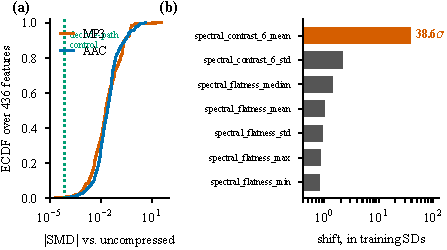
\includegraphics[width=\columnwidth]{figs/fig_mechanism.pdf}
\caption{What the codec does to the feature table, before any model is
involved. (a)~Empirical CDF of $|$SMD$|$ over all 436 features against
uncompressed audio, 7{,}441 clips: both codecs leave the median feature
untouched and differ only in the tail. The green line marks the decode-path
control median ($7.6\times10^{-5}$). (b)~The MP3 tail in \emph{training}
standard deviations: one descriptor of the 6--8\,kHz band moves 38.6$\sigma$,
the next largest 2.1$\sigma$.}
\label{fig:mech}
\end{figure}

\section{Method}
\subsection{Corpus and coding conditions}
We use CREMA-D~\cite{cao2014cremad}: 7{,}442 clips from 91 actors, each
delivering one of twelve fixed sentences in one of six acted emotions
(anger, disgust, fear, happiness, neutral, sadness); 5.26\,h of audio. The
fixed lexical inventory is load-bearing --- holding the words constant across
emotions removes the lexical channel as a source of discriminative variance, so
any recovered signal must be carried by acoustic realisation.

Every clip is rendered into four conditions descended from a single canonical
reference $x$ (16\,kHz mono 16-bit PCM, EBU~R128 normalised to $I=-23$\,LUFS,
TP${}=-2$\,dB): \ft{ref} ($x$ itself); \ft{mp3\_64} (libmp3lame, 64\,kbps);
\ft{mp4\_aac64} (AAC, 64\,kbps, audio-only MP4); and \ft{roundtrip\_wav}, the
AAC output decoded back to PCM through one identical FFmpeg call. Single
ancestry makes the format contrast the only systematic difference between
conditions, and a fixed decode path keeps the decoder from confounding the
codec.

\ft{roundtrip\_wav} is the container control: codec output held fixed while the
delivery wrapper changes, so any difference from \ft{mp4\_aac64} is
attributable to routing rather than coding. Its median standardised feature
difference from \ft{mp4\_aac64} is $7.6\times10^{-5}$, with only 12 of 436
features exceeding $0.05$ --- the noise floor of the study. Any effect larger
is a codec effect.

\subsection{Features}
Each file is reduced to 436 named descriptors, every frame-level contour
collapsed to eight order statistics (mean, median, SD, IQR, min, max, skew,
kurtosis). The families are \emph{spectral} (114: centroid, bandwidth, rolloff,
flatness, flux, entropy, slope, ZCR, RMS, seven-band spectral contrast, eight
band-energy ratios, and explicit high-frequency survival ratios above 4 and
6\,kHz), \emph{cepstral} (240: 20 MFCCs with $\Delta$ and $\Delta\Delta$),
\emph{prosodic} (56, computed in Praat via
Parselmouth~\cite{jadoul2018parselmouth}: $F_0$ statistics and slope, jitter,
shimmer, HNR, formants $F_1$--$F_5$ with bandwidths, intensity, voiced-segment
timing and cepstral peak prominence), \emph{chroma} (24) and two global
descriptors. Spectral and cepstral features use
librosa~\cite{mcfee2015librosa} at 512-point FFT, 160-sample hop. Chroma tuning
is pinned to zero rather than estimated, because an estimated tuning could
itself shift under compression and would silently become part of the effect
being measured.

Extraction over $7{,}442\times4$ files failed on exactly one clip in all four
conditions, \ft{1076\_MTI\_SAD\_XX}, which the corpus documentation lists as
having no audio; 7{,}441 clips form the analysis set.

\subsection{Models and protocol}
Actors are partitioned 60/11/20 into train, validation and test with sex
balance preserved, yielding 4{,}905/896/1{,}640 clips. Speaker-independent
splitting is not a nicety: a variance decomposition over the feature table gives
mean $\eta^2=0.178$ for speaker against $0.098$ for emotion, with 340 of 436
features speaker-dominant, so a random row split would leak voice identity into
the test set and inflate every score below.

Fourteen scikit-learn classifiers~\cite{pedregosa2011sklearn} spanning tree
ensembles~\cite{breiman2001rf,chen2016xgboost,ke2017lightgbm,friedman2001gbm},
kernel machines~\cite{cortes1995svm}, linear and discriminant models and
probabilistic baselines, plus a PyTorch~\cite{paszke2019pytorch} MLP
(512--256--128, batch normalisation, dropout 0.3; AdamW, $\text{lr}=10^{-3}$,
cosine schedule; class-weighted cross-entropy with label smoothing 0.05; early
stopping on validation UAR) --- fifteen trained models --- are fitted on
\ft{ref} and evaluated on all four conditions. Missing values are imputed with
training medians and scaling applied only where needed, so tree SHAP values
stay in interpretable physical units. The same clips appear in every condition,
so a cross-format comparison differs only in format.

For reference throughout: CREMA-D's crowd raters, hearing audio alone, matched
the intended emotion on 45.5\,\% of clips (per-class recall 0.966 for neutral
down to 0.164 for sad). Models trained on the \emph{intended} label can exceed
this by exploiting acting cues human listeners do not consciously decode; the
figure is context for absolute accuracy, not a target.

\subsection{Attribution}
Attribution is computed on the held-out speakers using TreeSHAP for the
ensembles~\cite{lundberg2020treeshap}, LinearSHAP for the linear models,
LIME~\cite{ribeiro2016lime}, permutation importance, partial dependence, a
depth-4 global surrogate tree, and, for the network, six methods from
Captum~\cite{kokhlikyan2020captum}: Saliency, Input$\times$Gradient, Integrated
Gradients, DeepLIFT, GradientSHAP and Feature Ablation. Cross-format stability
is Spearman $\rho$ between mean-$|$attribution$|$ rankings over all 436
features, reported with the number of top-25 features retained.

The RBF-SVM has no exact explainer and was given KernelSHAP with 100 sampled
coalitions over 436 features. That least-squares system is rank-deficient and
diverged (maximum mean $|$SHAP$|$ of $2.1\times10^{12}$ against a median of
$5.3\times10^{-4}$). Its KernelSHAP ranking is excluded from every attribution
conclusion here; the SVM contributes accuracy and robustness results only.

\section{Results}
\subsection{What the codec does to the features}
Fig.~\ref{fig:mech} characterises the manipulation before any model is
involved. Both codecs leave the median feature essentially untouched (median
$|$SMD$|$ 0.020 for MP3, 0.025 for AAC); the difference lives entirely in the
tail. Under MP3, 63 of 436 features exceed $|$SMD$|$ of 0.2 and 28 exceed 0.5,
but one descriptor dominates: \scsix, summarising the 6--8\,kHz band, moves by
38.6 training standard deviations against 2.1$\sigma$ for the next largest.
This is perceptual bit allocation seen from the feature side --- the encoder
abandons the top octave and one column reports it.

AAC's contribution differs in kind. Its largest shifts are all delta-MFCC means
(\ft{mfcc\_d1\_01\_mean}, ${\rm SMD}=-4.16$), consistent with encoder priming
shifting frame alignment uniformly: a small perturbation to every first-order
derivative rather than the destruction of one band. One caveat belongs with
that number --- delta means sit near zero with small standard deviations, so
their standardised shifts are inflated relative to absolute change.

\begin{table}[!t]
\caption{Balanced accuracy on 20 held-out speakers, all models trained on
uncompressed audio. Models are grouped by how the decision rule consumes a
feature value. Chance ${}=0.167$; human voice-only ${}=0.455$.
\ft{rt} is the container control (AAC re-wrapped as WAV).}
\label{tab:cross}
\centering
\scriptsize
\setlength{\tabcolsep}{3.2pt}
\begin{tabular}{@{}llccccc@{}}
\toprule
& Model & \ft{ref} & \ft{mp3} & $\Delta$ & \ft{aac} & \ft{rt} \\
\midrule
\multirow{7}{*}{\rotatebox{90}{\textit{thresholds}}}
& LightGBM        & 0.591 & 0.586 & $-0.005$ & 0.559 & 0.562 \\
& XGBoost         & 0.582 & 0.586 & $+0.004$ & 0.560 & 0.560 \\
& HistGB          & 0.573 & 0.559 & $-0.014$ & 0.530 & 0.533 \\
& Random forest   & 0.535 & 0.532 & $-0.003$ & 0.522 & 0.522 \\
& AdaBoost        & 0.521 & 0.511 & $-0.010$ & 0.487 & 0.484 \\
& Extra trees     & 0.519 & 0.521 & $+0.002$ & 0.512 & 0.507 \\
& Decision tree   & 0.390 & 0.382 & $-0.009$ & 0.367 & 0.371 \\
\midrule
\multirow{8}{*}{\rotatebox{90}{\textit{multiplies}}}
& $k$NN           & 0.479 & 0.362 & $-0.117$ & 0.467 & 0.457 \\
& Gaussian NB     & 0.430 & 0.277 & $-0.152$ & 0.437 & 0.433 \\
& Linear SVM      & 0.584 & 0.405 & $-0.179$ & 0.471 & 0.462 \\
& MLP             & 0.574 & 0.383 & $-0.191$ & 0.491 & 0.494 \\
& ANN (PyTorch)   & 0.599 & 0.354 & $-0.246$ & 0.513 & 0.512 \\
& LDA             & 0.585 & 0.338 & $-0.247$ & 0.507 & 0.502 \\
& Log.\ regression& 0.567 & 0.233 & $-0.334$ & 0.472 & 0.470 \\
& SVM (RBF)       & 0.586 & 0.203 & $\mathbf{-0.383}$ & 0.499 & 0.497 \\
\bottomrule
\end{tabular}
\end{table}

\begin{figure*}[!t]
\centering
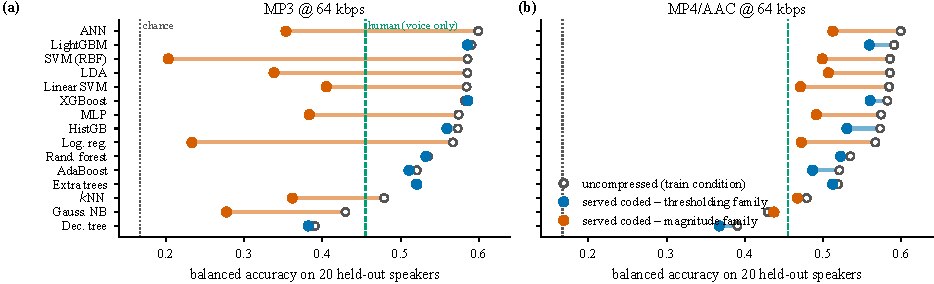
\includegraphics[width=\textwidth]{figs/fig_crossformat.pdf}
\caption{Robustness to lossy coding is determined by how a model consumes its
inputs, not by how accurate it is. Open circles are the uncompressed score,
filled circles the score when the same fitted model is served coded audio.
(a)~Under MP3 the two families separate completely: no thresholding model
moves more than 0.014, no magnitude model less than 0.117. Four magnitude
models fall below the human voice-only ceiling and one lands within
0.04 of chance. (b)~Under AAC the same models degrade broadly and mildly, and
the families interleave --- consistent with a diffuse frame-alignment
perturbation rather than a single-band blowout.}
\label{fig:cross}
\end{figure*}

\subsection{In-format performance}\label{sec:leaderboard}
Trained and tested on uncompressed audio (the \ft{ref} column of
Table~\ref{tab:cross}), the network leads at 0.599 balanced accuracy, with
LightGBM, the RBF-SVM, LDA and the linear SVM within two points. Two
observations matter, and neither is about the winner. The single decision tree
--- the one model a human can read end to end --- reaches 0.390 against 0.599,
so intrinsic interpretability costs a third of the achievable performance here:
an argument against Rudin's prescription~\cite{rudin2019stop} in this setting
and in favour of post-hoc attribution over a strong model. And the spread
across the top eight models is under three points, so the leaderboard ordering
carries little information. The differences that matter are 12 to 38 points and
appear only when the format changes.

\subsection{The family split}\label{sec:family}
Table~\ref{tab:cross} and Fig.~\ref{fig:cross} give the central result. Under
MP3 the outcome is categorical rather than graded. Every tree-based model sits
within $\pm0.014$ of its clean score --- two of them improve slightly. Every
model that consumes features as continuous magnitudes loses between 0.117 and
0.383. There is no overlap between the two groups and no intermediate case; the
gap between the worst thresholding model and the best magnitude model is a
factor of eight.

The partition does not track accuracy. The best and the worst MP3 performers
(the network at 0.599 clean and the decision tree at 0.390) sit on opposite
sides of it, and so do the second-best and third-best clean models (LightGBM,
$-0.005$; the RBF-SVM, $-0.383$). It does not track model capacity, linearity,
or whether the model is parametric. It tracks one thing: whether the decision
rule compares a feature to a constant or multiplies it by one.

Given \S4.1 the mechanism is immediate. A tree asks whether \scsix{} exceeds a
threshold near 17; the answer is unchanged whether the feature reads 16.4 or
46.4. A linear or kernel model multiplies that 38.6$\sigma$ excursion straight
into its decision function. This is textbook covariate
shift~\cite{morenotorres2012shift}, with one unusual property: the shifted
variable is not a proxy for anything the label depends on, so the shift is pure
contamination.

MP4/AAC behaves as its different mechanism predicts --- costing everyone
something and nobody very much (0.7 to 11.3 points, regardless of family) and
leaving the two groups interleaved rather than separated. Whatever governs
robustness, then, is an interaction between the codec's error structure and the
decision rule, not a property of either alone.

\textbf{The container is inert.} Across the fifteen models the median
difference between \ft{roundtrip\_wav} and \ft{mp4\_aac64} is 0.003 balanced
accuracy, with a maximum of 0.010 ($k$NN), against MP3 codec effects reaching
0.383 --- one to two orders of magnitude larger. For a feature pipeline that
decodes both routes itself this null is close to structural, and that is
precisely its value: confirming it is what licenses attributing everything else
to the codec.

\textbf{Matched-format training is a partial fix.} Trained on \ft{mp4\_aac64}
instead of \ft{ref}, the RBF-SVM scores 0.572 on AAC and logistic regression
0.570, against 0.586 and 0.567 clean-on-clean: the emotional information
survives 64\,kbps AAC intact, and what fails is the train/serve mismatch. But
training on AAC does not rescue MP3 --- the SVM falls to 0.167, exactly chance
--- so the fix is codec-specific, not a general immunisation.

\subsection{What the models attribute to}\label{sec:xai}
\subsubsection{Convergent evidence}
On uncompressed audio, five model families and four attribution algorithms
select the same acoustic evidence. The top SHAP features for XGBoost and
LightGBM are identical in the first five (\ft{mfcc\_d1\_00\_std},
\ft{mfcc\_d2\_00\_std}, \ft{duration\_s}, \ft{prosody\_intensity\_std},
\ft{mfcc\_00\_std}), and all six gradient methods on the network return the
first two plus \ft{prosody\_cpps} and \ft{duration\_s}. The two leaders are the
standard deviations of the first and second derivative of MFCC-0 --- how
variable the rate of change of overall loudness is, a direct formalisation of
vocal agitation. Per-emotion attributions are equally sensible: cepstral peak
prominence, a breathiness correlate, drives sadness and neutrality; $F_0$
median drives fear; $F_2$ movement drives disgust. The network was told none of
this.

\subsubsection{The methods disagree with each other}
Fig.~\ref{fig:xai}(a) is the uncomfortable result. SHAP tracks a model's
\emph{intrinsic} importance closely for the simpler models ($\rho=0.984$ for
the decision tree, $0.983$ for logistic regression), but LIME and permutation
importance are close to unrelated to it. On the decision tree, LIME and SHAP
rank features at $\rho=0.008$ --- no relationship at all --- while still
sharing 10 of their top 20. This reproduces the disagreement problem Krishna et
al.~\cite{krishna2022disagreement} document, on a model simple enough that no
approximation error can be blamed.

A within-family comparison sharpens rather than softens the point: the six
gradient methods on the network agree almost perfectly ($\rho\geq0.936$
pairwise, Integrated Gradients and DeepLIFT at $0.998$). High agreement
\emph{within} a
method family is therefore not evidence of correctness --- these methods share
a mathematical lineage, and their consensus reflects that lineage. A
single-method claim about which acoustic features matter is not reproducible
across methods; only features surviving all four independent views should be
reported, and here that set is \ft{mfcc\_d1\_00\_std},
\ft{prosody\_intensity\_std}, \ft{duration\_s}, \ft{prosody\_cpps} and
\ft{prosody\_f0\_median}.

Two calibrations belong with this result. A depth-4 global surrogate reproduces
its target model's predictions only 57--74\,\% of the time (random forest
73.9\,\%, LightGBM 63.4\,\%, XGBoost 62.1\,\%, SVM 58.7\,\%, decision tree
58.2\,\%, logistic regression 57.1\,\%), so surrogate rules summarise a
majority of a model, not a model. And the network's attributions pass the
model-randomisation check~\cite{adebayo2018sanity}
(Fig.~\ref{fig:xai}(b)): correlation between attributions from the trained
network and a randomly initialised one of identical architecture ranges from
$-0.011$ to $0.206$ across all six methods.

\begin{figure}[!t]
\centering
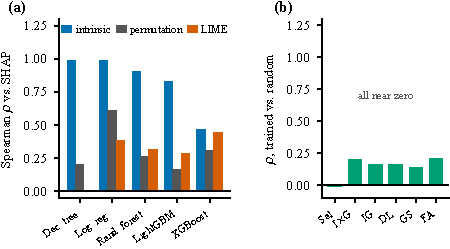
\includegraphics[width=\columnwidth]{figs/fig_xai.pdf}
\caption{Attribution diagnostics. (a)~Post-hoc methods compared against SHAP on
the same fitted tabular model, Spearman $\rho$ over all 436 features. SHAP
tracks intrinsic importance closely for the simpler models, but LIME and
permutation importance are nearly unrelated to it; on the decision tree LIME and
SHAP agree at $\rho=0.008$. (b)~Model-randomisation sanity check: all six
gradient methods are near zero against a randomly initialised network, so these
explanations describe the trained model rather than the input distribution.}
\label{fig:xai}
\end{figure}

\subsubsection{Stability under coding, and a blind spot}
Table~\ref{tab:stab} gives cross-format attribution stability. The ordering
follows the same family split as accuracy: tree and linear attributions barely
move under MP3 ($\rho\geq0.987$), while the network's fall to $\rho=0.677$ with
only 11 of its top 25 features retained.

What replaces what is readable only because the features are named. Under MP3
the features \emph{entering} the network's top 25 are almost all encoder
artefacts --- \ft{spectral\_flatness} in five statistics, plus \scsix{} ---
while the features \emph{leaving} are genuine voice-quality and prosodic
measures: \ft{prosody\_cpps}, \ft{prosody\_f0\_skew}, \ft{prosody\_f2\_mean},
\ft{prosody\_f2\_std}, \ft{prosody\_f3\_bw\_median}. The compressed model stops
listening to the voice and starts listening to the encoder.

The logistic regression row is the most important negative result here. Its
SHAP ranking is essentially unchanged under MP3 ($\rho=0.987$, 22 of 25 top
features retained) while its balanced accuracy collapses from 0.567 to 0.233.
The coefficients did not change; only the inputs went out of range, and a
global mean-$|$SHAP$|$ ranking is largely blind to that. \textbf{A global
attribution-stability metric can report ``nothing changed'' while the
classifier has stopped working.} Any deployment monitoring explanation
stability as a proxy for model health must pair it with input-range monitoring
or per-instance attribution.

\begin{table}[!t]
\caption{Attribution stability: Spearman $\rho$ over all 436 features against
the uncompressed condition, with top-25 features retained in parentheses. SHAP
for all rows except the ANN, which uses Integrated Gradients. The last column
repeats the MP3 accuracy change for comparison.}
\label{tab:stab}
\centering
\scriptsize
\setlength{\tabcolsep}{4pt}
\begin{tabular}{@{}lcccc@{}}
\toprule
Model & \ft{mp3\_64} & \ft{mp4\_aac64} & \ft{rt} & $\Delta$ acc.\ MP3 \\
\midrule
Decision tree       & 0.995 (24) & 0.988 (21) & 0.988 (21) & $-0.009$ \\
XGBoost             & 0.991 (25) & 0.984 (22) & 0.984 (22) & $+0.004$ \\
Random forest       & 0.990 (25) & 0.976 (25) & 0.975 (25) & $-0.003$ \\
LightGBM            & 0.988 (23) & 0.983 (22) & 0.982 (22) & $-0.005$ \\
Log.\ regression    & 0.987 (22) & 0.942 (21) & 0.941 (21) & $\mathbf{-0.334}$ \\
ANN (Int.\ grad.)   & \textbf{0.677 (11)} & 0.891 (16) & 0.887 (16) & $-0.246$ \\
\bottomrule
\end{tabular}
\end{table}

\subsection{Diagnosis and repair}\label{sec:repair}
Because the features are named, the failure is not merely observable but
addressable. Features were ranked by how far each codec moves them in units of
\emph{training} standard deviation, then progressively replaced with training
medians in both the compressed and the clean test set --- the clean column
controlling for whatever real signal the masking itself destroys.

Fig.~\ref{fig:neut} gives the outcome. The single masked feature is \scsix.
Masking it alone lifts the RBF-SVM from 0.203 to 0.577 and the network from
0.354 to 0.580 --- recovering 97.9\,\% and 92.3\,\% of their respective losses
--- and three features bring logistic regression to 0.562 against its 0.567
clean-audio score. The tree models are flat throughout, having had nothing to
recover.

Two controls make this a diagnosis rather than a coincidence. On uncompressed
audio the identical masking costs nothing out to 20 features --- the network's
clean control sits at 0.606--0.609, marginally \emph{above} its 0.599 unmasked
baseline --- so these columns were never load-bearing evidence; they were the
channel through which the encoder's fingerprint entered the model. And the AAC
case behaves as its diffuse mechanism predicts: no single feature dominates,
and recovery is gradual, the network peaking at 10 features masked
($0.513\rightarrow0.560$) and the SVM at 40 ($0.499\rightarrow0.542$).

The diagnosis is therefore covariate shift on a small set of identifiable
descriptors, not loss of emotional information. The ordering of remedies
follows: use a threshold-based model family, which is free; or clamp the
top-band spectral descriptors, which recovers almost everything at the cost of
one feature; or retrain on the target codec, which works but requires knowing
the codec in advance and does not transfer between codecs.

\begin{figure}[!t]
\centering
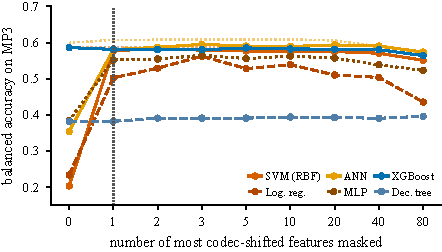
\includegraphics[width=\columnwidth]{figs/fig_neutralise.pdf}
\caption{Neutralisation under MP3: replacing the most codec-shifted features
with their training medians, ranked by shift in training standard deviations.
Masking one feature recovers almost the entire collapse for every affected
model; the tree models were never affected and are flat throughout. Beyond
roughly 20 features the masking begins to destroy real evidence. Dotted lines
show the same masking applied to uncompressed audio, where out to 20 features
it costs nothing.}
\label{fig:neut}
\end{figure}

\section{Discussion}
The practical recommendation is cheap and specific. A SER pipeline that will
encounter heterogeneous ingestion formats should either use a thresholding
model family, which costs nothing and removes the failure entirely, or monitor
and clamp the input range of its most codec-sensitive descriptors. Both are
available before any retraining is considered, and both are discoverable only
if the features carry acoustic names.

The result also resolves an apparent tension in the literature. Reddy and
Vijayarajan~\cite{reddy2020compression} report modest, front-end-dependent
codec effects on SER; we report catastrophic effects for half our models. Both
are correct. The magnitude of a codec effect is not a property of the codec,
and reporting it without specifying the model family is reporting an average
over a bimodal distribution --- which is what our Table~\ref{tab:cross} shows
the distribution to be.

More broadly, explanation stability is a reportable robustness property
distinct from accuracy but not a substitute for it. The two move together in
rank order here, yet each misses what the other catches: accuracy change
consistently \emph{under}-reports attribution change (XGBoost loses 2.2 points
on AAC while swapping 3 of its top 25 features; the network loses 8.7 while
swapping 9), while in the logistic regression case attribution change
dramatically under-reports accuracy collapse. Neither dominates, which is why
both belong in a robustness report, alongside the reporting standards urged for
ML-based science generally~\cite{kapoor2024reforms}.

\subsection{Limitations}
Results come from a single deterministic actor partition rather than repeated
cross-validation, so leaderboard differences of a point or two should not be
over-read; the codec effects are 12--38 points and are not at risk from split
variance. Only 64\,kbps was tested per codec, and the MP3 result is severe
partly \emph{because} 64\,kbps is aggressive for that codec, so the bitrate at
which the family split appears is not established here. Every frame contour is
collapsed to order statistics, so no attribution localises \emph{when} in the
clip the evidence sits, and attribution comparisons are global --- which
\S\ref{sec:xai} shows can miss a total accuracy collapse. Finally, the corpus
is acted English from one dataset, and its 45.5\,\% human voice-only ceiling
shows the labels are only loosely recoverable from audio; absolute accuracies
do not transfer to spontaneous speech.

\section{Conclusion}
Serving a speech emotion model coded audio it was not trained on costs between
nothing and two thirds of its headroom above chance, and which of those you get
is decided by the model family, not the codec. Under 64\,kbps MP3 the split is
clean: from bit-identical inputs, thresholding models move by at most 0.014
balanced accuracy and magnitude models by at least 0.117. The cause is a single
named descriptor of the 6--8\,kHz band arriving 38.6 training standard
deviations out of range, and masking that one column recovers almost the entire
loss at no cost on clean audio; the container contributes nothing. Two
recommendations follow: report the delivery format, an experimental degree of
freedom currently going unrecorded, and report codec robustness per model
family rather than as an average, because the average describes none of the
models it summarises.

\section{Data availability and declarations}
\scriptsize\noindent
CREMA-D is public under the terms in~\cite{cao2014cremad}. All derived
artefacts are released: stimulus scripts and condition manifests, the
timestamped 436-feature table over 29{,}768 rendered files with its schema, the
fitted pipelines, and the result files from which every table and figure here
is generated; the figure script reads only these and hard-codes no reported
value. The study involves no human subjects and no personally identifying data,
uses a published corpus of consenting actors released under its authors' own
ethical approval, and made no new recordings; SER is dual-use, and these
findings are if anything cautionary about deployment without format-aware
validation. \textbf{CRediT}: A.~R --- conceptualization, methodology, software,
validation, formal analysis, investigation, data curation, writing,
visualization. \textbf{Conflicts}: none. \textbf{Funding}: none; compute costs
were borne by the author. \textbf{Generative AI} assisted with code, figures
and drafting; all design decisions, analyses and interpretations are the
author's, every reported value was produced by the committed pipeline, and
every citation was verified against a Crossref DOI record or the arXiv API.
\normalsize

\balance
\footnotesize
\bibliographystyle{IEEEtran}
\bibliography{refs}

\end{document}
